\chapter{Anticipated contribution} \label{contribution}
As the main contribution of my research to the software engineering and especially software process community I am envisioning development of a previously unexplored approach of discovering recurrent behaviours in software process using data mining of low-level process and product artifacts. This approach potentially may lead to the discovery of unknown patterns in software process and improve our knowledge about it.

Secondly, in order to validate the approach taken, I am working on the implementation of the software system called TrajectoryBrowser which will aid the discovery of the recurrent patterns. This system will provides means for real-valued data conversion into symbolic temporal format, its storage and indexing. The data-mining algorithms working with this data will be developed with expandable mechanism for search space pruning based on the domain knowledge base. Delivery of such a system will not only extend the functionality of the Hackystat but will provide a useful tool for mining any software process. Figure \ref{fig:system_overview} shows the overview of the future system.

Based on the previous work done 





I am working on implementing Implemented algorithms and methods for mining of temporal data. 

. providing aggreagtion and conversion of the low-level software process data into the symbolic temporal time-points and time-interval series. 


alloexperimental data mining, I am developing a Hackystat ExtensionAs the main tool for testing my ideas and perform experiments I am planning to develop working application of the previously unexplored approach community In summary, the proposed contributions of my research will include: 


\begin{itemize}
	\item the implementation of a system aiding in discovery of novel software process knowledge through the analysis of fine-grained software process and product data;
	\item experimental evaluation of the system, which will provide insight into its strengths and weaknesses;
	\item the potential discovery of useful new software process patterns.
\end{itemize}

\begin{figure}[tbp]
   \centering
   \includegraphics[height=65mm]{system_overview.eps}
   \caption{The high-level system overview. Software engineering process and product data collected and aggregated by Hackystat used to generate temporal symbolic indexes. Data mining tools constrained by the software engineering domain knowledge are then used for unsupervised patterns discovery. The GUI provides an expert interface for discovered patterns and knowledge base aiding iterative investigation of a discovered phenomena.}
   \label{fig:system_overview}
\end{figure}
